{$\space$\par}
\vspace{0.5cm}
\justifying
\section*{{\bfseries \LARGE Questão 6 -} {\bfseries \large Compare graficamente as distribuições de desvio para o vermelho (z) para cada classe (isto é, Type). A partir dessa comparação, descreva qualitativamente as diferenças encontradas.}}

\vspace{0.8cm}

\textcolor{red}{Para comparar as distribuições, fiz um histograma de cada tipo, mantendo os bins iguais para facilitar a visualização.}

\vspace{0.4cm}

\begin{lstlisting}
    data = read.table('/content/QSOBLC.dat', header=T, sep='|')
    
    par(mfrow=c(3,1))
    for (tip in c('QSO', 'SY1', 'BLZ')) {
      subset = data[data$Type == tip, ]
      hist(subset$z, breaks=seq(0,max(na.omit(data$z)+0.1), by=0.1), xlab = "Redshift z", xlim = c(0,max(na.omit(data$z))+0.1), main=tip, cex.main=2, cex.lab=1.5)
    }
\end{lstlisting}

\vspace{0.4cm}

\begin{figure}[h]
    \centering
    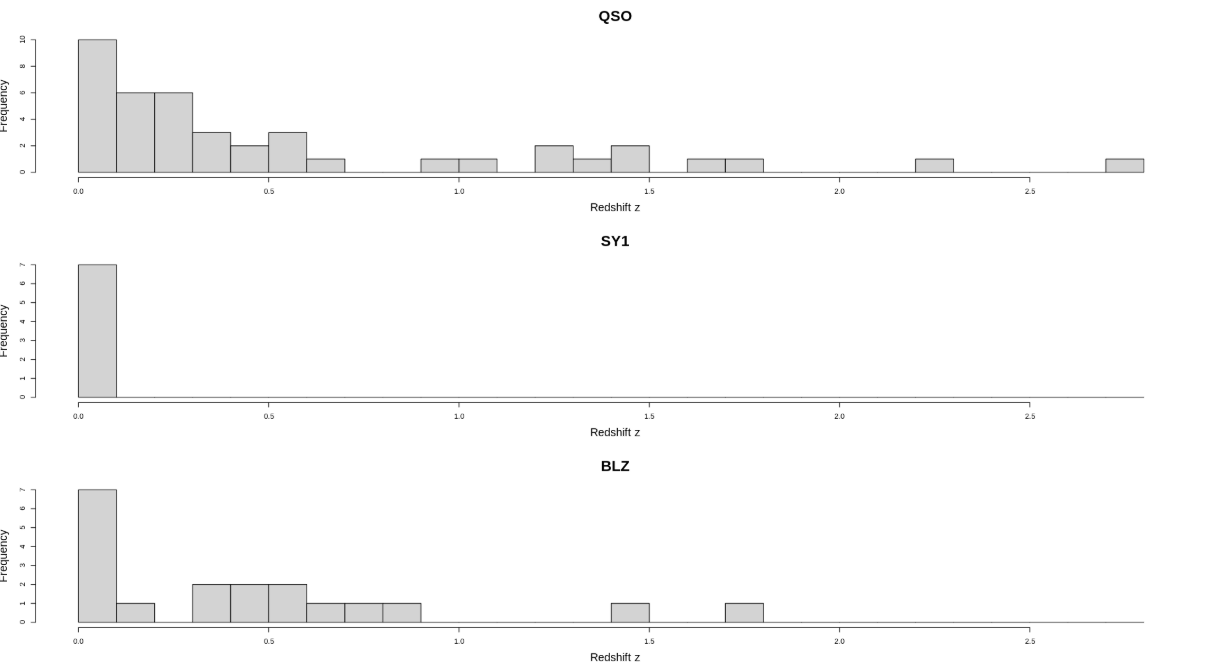
\includegraphics[width=0.9\linewidth]{Figuras/Captura de tela 2025-06-01 130405.png}
    \caption{Distribuição de redshift para quasares, galáxias Seyfert 1 e blazares do catálogo dado.}
\end{figure}

\textcolor{red}{Analisando os gráficos, podemos dizer que galáxias do tipo Seyfert 1 são objetos próximos à nossa galáxia, pois eles tem um baixo redshift. Além disso, pode-se observar semelhanças entre quasares e blazares.}